\documentclass[oneside]{uffstex}
\usepackage[utf8]{inputenc}
\usepackage[utf8]{inputenc}
\usepackage[T1]{fontenc}
\usepackage{float}
\usepackage{emptypage}
\usepackage[table]{xcolor}

\usepackage[style=abnt-numeric]{biblatex}
\addbibresource{refs.bib}
%======================CAPA========================

\titulo{CONTROLADOR DE BARRAMENTO}
\subtitulo{SISTEMAS DIGITAIS}
\autor{docente: GEOMAR ANDRE SCHREINER \\discentes: ARTHUR EMANUEL DA SILVA (2211100029)\\ E JÉSSICA BRITO DA SILVA (20240002517)}
\curso{Ciência da Computação}
\cidade{Chapecó}
\uf{SC}
%==========PALAVRAS CHAVE =======
\palavrachave{palavra chave}
\palavrachave{palavra chave}
\palavrachave{palavra chave}

\begin{document}
\imprimircapa%

%===============================SUMARIO===================================%
\pdfbookmark{\contentsname}{toc}
\tableofcontents*
\cleardoublepage%

%===============================CAPITULO 1=============================%
\textual%
\chapter{Introdução}
\section{Resumo}
Este relatório descreve o desenvolvimento de um sistema de arbitragem de barramento para quatro dispositivos de entrada e saída (disp0 a disp3), com controle de prioridade e lógica de concessão baseada em sinais de requisição ("req") e autorização ("aut"). O sistema implementa uma lógica que garante que o dispositivo com maior prioridade receba acesso preferencial ao barramento, com um botão que permite interromper a execução atual para conceder imediatamente o barramento a um dispositivo com prioridade superior. O projeto foi desenvolvido em linguagem VHDL e implementado fisicamente em uma placa FPGA, validando seu funcionamento conforme o esperado.
\section{Descrição do problema}
O controle de acesso ao barramento é um aspecto fundamental em sistemas digitais que envolvem múltiplos dispositivos compartilhando um mesmo canal de comunicação. Este projeto tem como objetivo implementar, em VHDL, um sistema de arbitragem para gerenciar o acesso de quatro dispositivos de entrada e saída (disp0, disp1, disp2 e disp3) a um barramento comum. A arbitragem obedece a uma hierarquia fixa de prioridades, sendo disp0 o mais prioritário e disp3 o menos prioritário.

Cada dispositivo possui um sinal de requisição ("req") e recebe do árbitro um sinal de autorização ("aut") que permite o acesso ao barramento. A autorização é concedida na borda ativa do sinal de relógio e permanece ativa enquanto a requisição estiver presente. O sistema também conta com um botão de prioridade, que, quando ativado, garante que o barramento seja imediatamente cedido ao dispositivo com maior prioridade entre os que estiverem requisitando.

O código foi escrito em VHDL, utilizando o editor Visual Studio Code (versão 1.100.2), em ambiente Ubuntu 24.04.2 LTS, com kernel 6.11.0-26-generic. A simulação, validação e síntese do projeto foram realizadas na ferramenta Intel Quartus. O sistema foi implementado fisicamente em uma placa FPGA ALTERA DE1, permitindo a verificação prática do seu funcionamento em hardware real, assegurando conformidade com os requisitos de temporização e lógica definidos.
\chapter{Estratégia de resolução}
Para solucionar o problema apresentado, foi desenvolvida uma Máquina de Estados Finita (FSM – Finite State Machine) que gerencia o controle de acesso ao barramento. A FSM garante o funcionamento correto do sistema, respeitando a hierarquia de prioridades dos dispositivos e as regras de concessão e liberação do barramento. A partir da FSM, é derivada a tabela de transições do problema, para facilitar sua implementação dentro dos process em VHDL.

\section{Máquina de estados do problema}
A máquina é composta por estados que representam o sistema em repouso (estado "idle") e os estados de autorização para cada um dos dispositivos (aut0, aut1, aut2, aut3). As transições entre esses estados ocorrem com base nos sinais de requisição (req) de cada dispositivo e no estado do botão de prioridade.

Abaixo está representada a FSM desenvolvida para este projeto:
\begin{figure}[H]
    \centering
    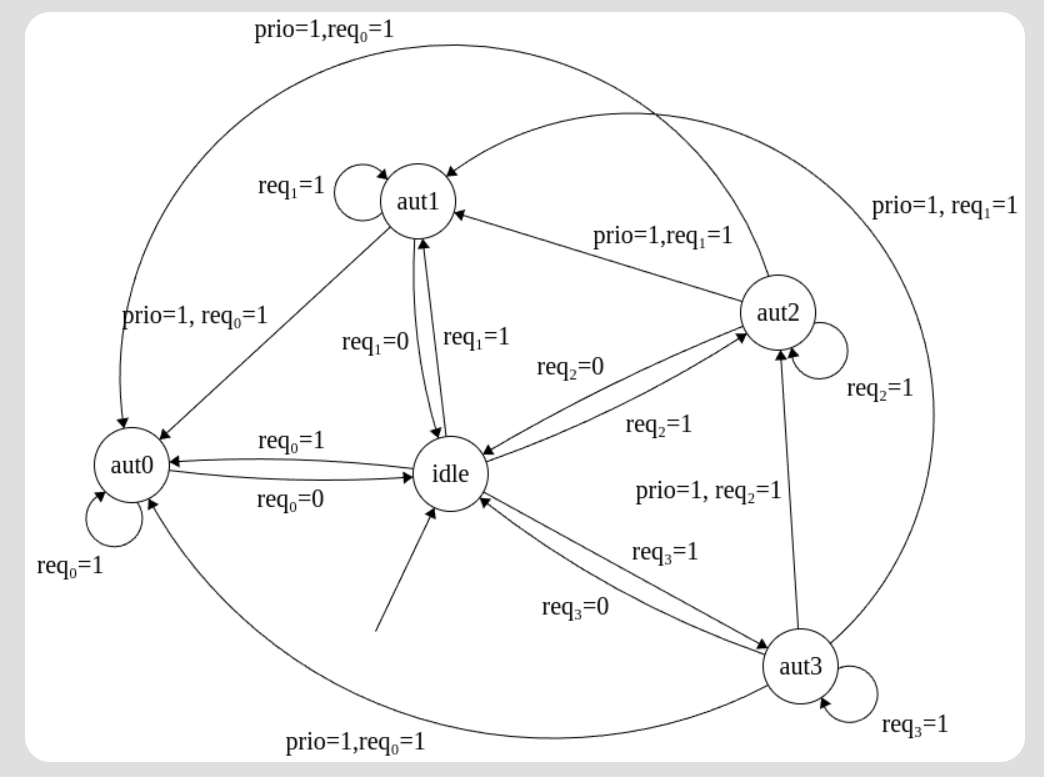
\includegraphics[width=0.9\linewidth]{morte.png}
    \caption{FSM do problema sugerido}
    \label{fig:FSM}
\end{figure}
Com base na FSM apresentada, o estado inicial e de repouso do sistema é o estado "idle". Em situações de entrada simultânea - por exemplo, se houver múltiplas requisições em uma entrada como "1001" a partir do estado idle — o comportamento definido é conceder acesso ao processo com maior prioridade entre aqueles que solicitam acesso, independente do botão de prioridade estar ou não ligado.

Quando o botão de prioridade está desativado, o dispositivo que estiver utilizando o barramento só libera o acesso ao retornar o sinal "reqX" para 0, independentemente do estado dos demais dispositivos. As transições para o estado idle ocorrem assim que o sinal de requisição do dispositivo atualmente autorizado for desativado, garantindo uma liberação ordenada do barramento.

Quando o botão de prioridade está ativado, o dispositivo que estiver utilizando o barramento só libera o acesso ao identificar o sinal "reqX" para algum dispositivo "reqN", respeitando a prioridade: disp0 > disp1 > disp2 > disp3. Dessa forma, partindo de disp3, é possível ir para disp2 (0011), disp1 (0101) e disp0 (1001), por exemplo.

Em cada transição envolvendo reqX=1, as req(X-n) de maior prioridade na escala estarão implicitamente como req(X-n)=0, pois a transição reqX=1 só ocorrerá quando todas as requisições de maior prioridade estiverem em 0, essa informação será omitida para simplificar a ilustração da Máquina de Estados, porém estará contemplada no Diagrama de estados na Tabela \ref{tab:diagramaestados}.
\section{Diagrama de transição de estados}

Com base na máquina de estados finita apresentada na seção anterior (Figura~\ref{fig:FSM}), foi derivado o diagrama de transição de estados, representado na Tabela~\ref{tab:diagramaestados}. Essa tabela descreve, para cada estado atual e combinação de entradas (req0 a req3 e priority), qual será o próximo estado do sistema. A abordagem adotada respeita a lógica de prioridade dos dispositivos e o comportamento do sistema tanto com o botão de prioridade ativado quanto desativado.

\begin{table}[H]
    \centering
    \caption{DIAGRAMA DE PRÓXIMO ESTADO}
    \begin{tabular}{|p{2cm}|p{1cm}|p{1cm}|p{1cm}|p{1cm}|p{2cm}|p{2cm}|}
        \hline
        CURRENT & req0 & req1 & req2 & req3 & priority & NEXT \\ 
        \hline
        idle & 0 & 0 & 0 & 0 & X & idle \\
        \hline
        idle & 1 & X & X & X & X & aut0 \\
        \hline
        aut0 & 1 & X & X & X & X & aut0 \\
        \hline
        aut0 & 0 & X & X & X & X & idle \\
        \hline
        idle & 0 & 1 & X & X & X & aut1 \\
        \hline
        aut1 & X & 1 & X & X & 0 & aut1 \\
        \hline
        aut1 & X & 0 & X & X & 0 & idle \\
        \hline
        aut1 & 1 & X & X & X & 1 & aut0 \\ 
        \hline
        aut1 & 0 & X & X & X & 1 & aut1 \\ 
        \hline
        idle & 0 & 0 & 1 & X & X & aut2 \\
        \hline
        aut2 & X & X & 1 & X & 0 & aut2 \\
        \hline
        aut2 & X & X & 0 & X & 0 & idle \\
        \hline
        aut2 & 1 & X & X & X & 1 & aut0 \\
        \hline
        aut2 & 0 & 1 & X & X & 1 & aut1 \\
        \hline
        idle & 0 & 0 & 0 & 1 & X & aut3 \\
        \hline
        aut3 & X & X & X & 1 & 0 & aut3\\
        \hline
        aut3 & X & X & X & 0 & 0 & idle\\
        \hline
        aut3 & 1 & X & X & X & 1 & aut0\\
        \hline
        aut3 & 0 & 1 & X & X & 1 & aut1\\
        \hline
        aut3 & 0 & 0 & 1 & X & 1 & aut2\\
        \hline
    \end{tabular}
    \label{tab:diagramaestados}
\end{table}

A Tabela~\ref{tab:diagramaestados} evidencia o comportamento determinístico da FSM frente às combinações possíveis de sinais de requisição e ao valor do botão de prioridade. Quando a prioridade está desativada (priority = 0), o dispositivo que está com o barramento mantém o controle até liberar voluntariamente (reqX = 0). Quando a prioridade está ativada (priority = 1), a FSM força a transição para o estado do dispositivo com maior prioridade que esteja com o sinal de requisição ativo. Esse comportamento assegura que o barramento esteja sempre sob controle do dispositivo mais prioritário entre os que estão solicitando acesso, de acordo com a lógica definida.
Para todos os processos listados acima, está implicitamente considerado o reset desligado. Quando o sinal de reset é detectado, o sistema retorna para o estado de idle.  
\chapter{Resolução}
\section{Planejamento do problema}
A interpretação que tivemos de como resolver situação problema do controlador de acesso a barramentos foi a seguinte:
\begin{figure}[H]
    \centering
    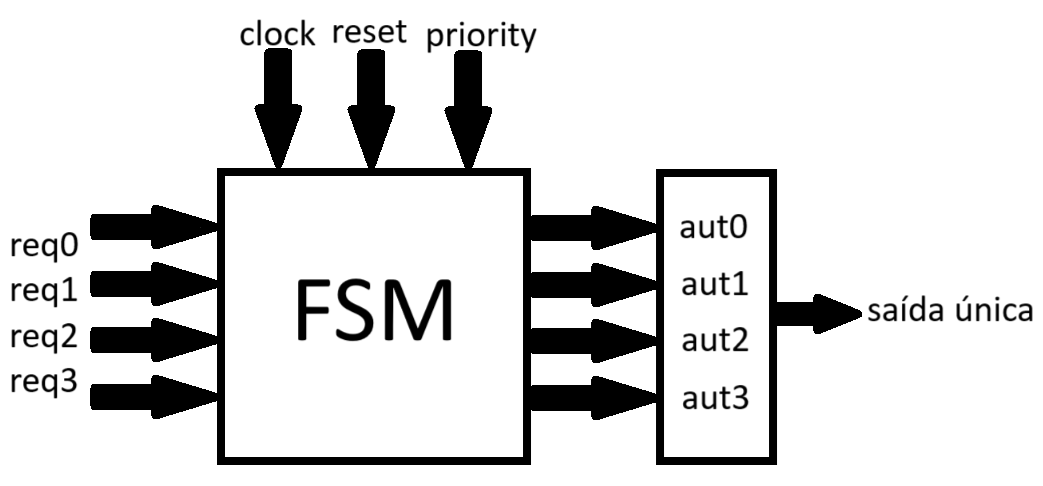
\includegraphics[width=0.9\linewidth]{PLANNING.png}
    \caption{Planejamento de solução}
    \label{fig:planejamento}
\end{figure}
Analisamos os req (de 0 a 3) juntamente dos clock, reset e priority. Eles tem o comportamento definido pela máquina de estados na Figura~\ref{fig:FSM} construída anteriormente e, com base nas possibilidades de entradas que temos, a FSM define se transiciona para algum dos estados (de aut0 à aut3) ou se mantém em idle (todos os aut zerados).
\subsection{Código conceitual}
Para essa parte da resolução, foi desenvolvido um código em VHDL com os elementos definidos acima, onde conceitualmente definimos clock, priority e demais entidades dentro do código, a fim de definir seu comportamento. Esse arquivo pode ser encontrado em anexo juntamente do código VHDL que possui as entradas devidamente mapeadas para sua implementação na FPGA posteriormente.
\subsection{ENTIDADE}
Para implementar o sistema em VHDL e, posteriormente, realizar sua execução na FPGA, foi necessário definir a entidade principal com base na arquitetura esquemática previamente desenvolvida. A Figura~\ref{fig:entidade} apresenta a descrição da entidade, com a especificação das entradas e saídas utilizadas no projeto.
Para implementar nosso programa em VHDL e posteriormente aplicá-lo na FPGA, com base na esquemática desenvolvida acima, definimos as entradas e saídas da entidade como sendo as seguintes
\begin{figure}[H]
    \centering
    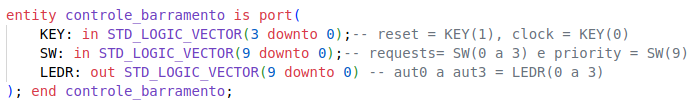
\includegraphics[width=1.0\linewidth]{ENTITY.png}
    \caption{Entidade no código VHDL}
    \label{fig:entidade}
\end{figure}
A entidade possui quatro sinais de saída (aut0 a aut3), os quais indicam qual dispositivo está autorizado a utilizar o barramento. Na implementação física com a FPGA, esses sinais são representados por LEDs. Como entradas, há um vetor que representa os sinais de requisição dos dispositivos (req0 a req3) e determina as transições de estado. A entrada priority define o modo de arbitragem: quando em nível lógico '0', o dispositivo atual mantém o barramento até liberar; quando em '1', o sistema verifica se há um dispositivo de maior prioridade requisitando acesso. Por fim, a entrada reset tem como função retornar o sistema ao estado inicial (idle), independentemente da situação corrente.

\subsection{Arquitetura}
O comportamento da entidade foi definido com base no diagrama desenvolvido previamente (Figura~\ref{fig:planejamento}), utilizando as entradas da entidade e aplicando-as dentro de dois blocos process distintos na descrição VHDL. O objetivo principal foi implementar fielmente a lógica de transições de estado apresentada na Tabela~\ref{tab:diagramaestados}, bem como o controle das saídas correspondentes. 
\begin{figure}[H]
    \centering
    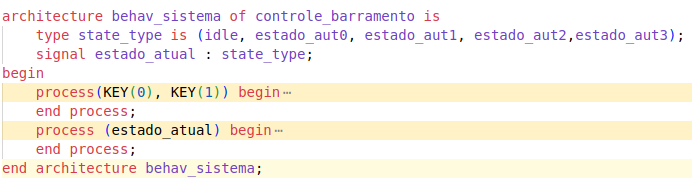
\includegraphics[width=0.9\linewidth]{ARCHITECTURE.png}
    \caption{Arquitetura da entidade no código VHDL}
    \label{fig:arquitetura}
\end{figure}
O primeiro process é responsável pela lógica de transição de estados. Nele, o estado atual retorna para idle sempre que o sinal de reset for detectado. Caso o reset não seja detectado e ocorra uma borda de subida no sinal de clock, a transição de estado é executada conforme as regras definidas na tabela de transições.

O segundo process trata exclusivamente das saídas da entidade, ou seja, dos sinais aut0 a aut3. Cada uma dessas saídas é ativada ou desativada de acordo com o estado atual, refletindo diretamente qual dispositivo está autorizado a acessar o barramento em determinado momento.

\section{Implementação na FPGA}
A implementação física do algoritmo foi realizada na UNIVERSITY PROGRAM ALTERA DEVELOPMENT\& EDUCATION BOARD DE1 EP2C20F484C7NK, executado pelo Quartus Cyclone II  no ambiente do Windows 10, onde as variáveis da situação problema foram mapeadas da seguinte forma:
\begin{table}[H]
    \centering
    \begin{tabular}{|c|c|}
    \hline
        variáveis VHDL & mapeamento FPGA \\
        \hline        
        clock & KEY(0) \\
        \hline
        reset & KEY(1) \\         
        \hline
        request(0) & SW(0) \\
        \hline
        request(1) & SW(1) \\ 
        \hline
        request(2) & SW(2) \\ 
        \hline
        request(3) & SW(3) \\         
        \hline
        priority & SW (9) \\
        \hline
        aut0 & LEDR(0) \\ 
        \hline
        aut1 & LEDR(1) \\
        \hline
        aut2 & LEDR(2) \\
        \hline
        aut3 & LEDR(3) \\
        \hline
    \end{tabular}
    \caption{Mapeamento na placa FPGA}
    \label{tab:mapeamento}
\end{table}
Verificamos que o árbitro funcionou corretamente ao selecionar o processo mais prioritário para acesso ao barramento, mesmo com múltiplos solicitantes estavam no estado 'IDLE'. Além disso, demonstrou-se que, se o botão de prioridade estivesse ativado e um processo de maior prioridade fosse requisitado durante a execução de um processo inicial, o sistema interrompe este último na próxima subida do clock para permitir que o processo de maior prioridade acesse o barramento, seguindo o comportamento esperado pela FSM na Figura \ref{fig:FSM}.


\chapter{Conclusão}
A resolução proposta neste trabalho lida com as ocasiões em que o barramento se encontra em modo de espera, inicializando o processo de maior prioridade que requisitar acesso ao barramento na borda de subida do clock, sendo essa ativação realizada manualmente por meio de um botão na FPGA. Além do funcionamento no estado Idle, também é utilizado um botão de prioridade, que permite que um processo em execução seja interrompido para dar lugar a outro com prioridade superior, dentro do contexto da aplicação. Ou seja, o processo 4 pode ter sua execução interrompida para ceder o barramento ao processo 3, caso este solicite acesso e possua maior prioridade. No entanto, o oposto não é verdadeiro: uma vez que o processo 3 tem prioridade superior ao processo 4, este último jamais obterá acesso ao barramento enquanto o modo de prioridade estiver ativado e o processo 3 continuar realizando requisições.

Entretanto, a ausência de uma pilha nesse contexto contexto impõe uma limitação importante: caso um processo A tenha sua execução interrompida por um processo B de maior prioridade, o barramento não retoma automaticamente a execução de A ao término de B. Em vez disso, no próximo ciclo de clock, o árbitro apenas concederá acesso novamente a A se ele ainda for o processo de maior prioridade ativo naquele momento. Dessa forma, não há garantia de continuidade imediata para processos previamente interrompidos, comprometendo a preservação da ordem original de execução em cenários com múltiplas prioridades.
\end{document}
 